%Metroplolis Beamer Theme: https://github.com/matze/mtheme
\documentclass[aspectratio=169, 10pt, dvipsnames, handout]{beamer}
\usetheme{metropolis}
\usepackage{appendixnumberbeamer, lmodern, bookmark,fontawesome}
\usepackage{booktabs}
% \usepackage[sorting=none]{biblatex}
\usepackage[scale=2]{ccicons}
\usepackage{pgfplots}
\usepgfplotslibrary{dateplot}
\usepackage{xspace}
\newcommand{\themename}{\textbf{\textsc{metropolis}}\xspace}
\usepackage{bbm}
\usepackage{tikz, graphicx}
\usepackage{caption, subcaption}
\usepackage{multicol}
% \usepackage[dvipsnames]{xcolor}
\usepackage{animate}
\usepackage{scalerel,xparse}
\usepackage{amsmath}
\usepackage[style=british]{csquotes}

\title{Progress update}
% \subtitle{Lab Update}
\date{\today}
\author{Philip Hartout}

% \titlegraphic{\hfill\includegraphics[height=1.5cm]{logo.pdf}}

\hypersetup{
  colorlinks=true,
  linkcolor=orange,
  filecolor=orange,
  urlcolor=orange,
}

\def\signed #1{{\leavevmode\unskip\nobreak\hfil\penalty50\hskip1em
  \hbox{}\nobreak\hfill #1%
  \parfillskip=0pt \finalhyphendemerits=0 \endgraf}}

\newsavebox\mybox
\newenvironment{aquote}[1]
  {\savebox\mybox{#1}\begin{quote}\openautoquote\hspace*{-.7ex}}
  {\unskip\closeautoquote\vspace*{1mm}\signed{\usebox\mybox}\end{quote}}

\titlegraphic{%
  
\includegraphics[width=.2\textwidth]{figures/mlcb-transparent.png}\hfill
  
\includegraphics[width=.2\textwidth]{figures/dbsse-transparent.png}\hfill
  
\includegraphics[width=.2\textwidth]{figures/eth-transparent.png}
}

\makeatletter
\setbeamertemplate{title page}{
  \begin{minipage}[b][\paperheight]{\textwidth}
    \vfill%
    \ifx\inserttitle\@empty\else\usebeamertemplate*{title}\fi
    \ifx\insertsubtitle\@empty\else\usebeamertemplate*{subtitle}\fi
    \usebeamertemplate*{title separator}
    \ifx\beamer@shortauthor\@empty\else\usebeamertemplate*{author}\fi
    \ifx\insertdate\@empty\else\usebeamertemplate*{date}\fi
    \ifx\insertinstitute\@empty\else\usebeamertemplate*{institute}\fi
    \vfill
    \ifx\inserttitlegraphic\@empty\else\inserttitlegraphic\fi
    \vspace*{1cm}
  \end{minipage}
}
\makeatother

\usetikzlibrary{shapes.geometric, arrows}

\tikzstyle{orangebox} = [rectangle, rounded corners, minimum width=2cm, minimum height=0.5cm, draw=black, fill=orange!40]
\tikzstyle{bluebox} = [rectangle, rounded corners, minimum width=2cm, minimum height=0.5cm, draw=black, fill=blue!40]

\tikzstyle{arrow} = [thick,->,>=stealth]


\begin{document}

\maketitle

\begin{frame}[fragile]{Introduction}


  \begin{itemize}
  \item W-L implementation
  \item Go through MMD code
  \item Discuss distances with TDA representations
  \item Some biological considerations for later
  \end{itemize}
\end{frame}

\begin{frame}[fragile]{Linear kernel}
  \begin{itemize}
  \item Not much to optimize there.
  \end{itemize}
\end{frame}


\begin{frame}[fragile]{Weisfeiler-Lehmann kernel}
  \begin{itemize}
  \item Computing $\phi(G)$ needs to be done explicitely and can be done
    independently (and in parallel) prior to computing $K_{WL}=\phi(G)^T\phi(G')$
  \item How to compute $\phi(G)$? \texttt{networkx} has a function called
    \href{https://networkx.org/documentation/stable/reference/algorithms/generated/networkx.algorithms.graph_hashing.weisfeiler_lehman_subgraph_hashes.html?highlight=weisfeiler_lehman_subgraph_hashes#networkx.algorithms.graph_hashing.weisfeiler_lehman_subgraph_hashes}{\texttt{weisfeiler\_lehman\_subgraph\_hashes}}.
  \item Since we don't care about the order in the resulting
    $K_{WL}=\phi(G)^T\phi(G')$, we can list each product that needs to be done
    and execute them in parallel as well.
  \end{itemize}
\end{frame}


\begin{frame}[fragile]{Weisfeiler-Lehmann kernel}
  What does the implementation look like?
  \begin{figure}
    \centering
    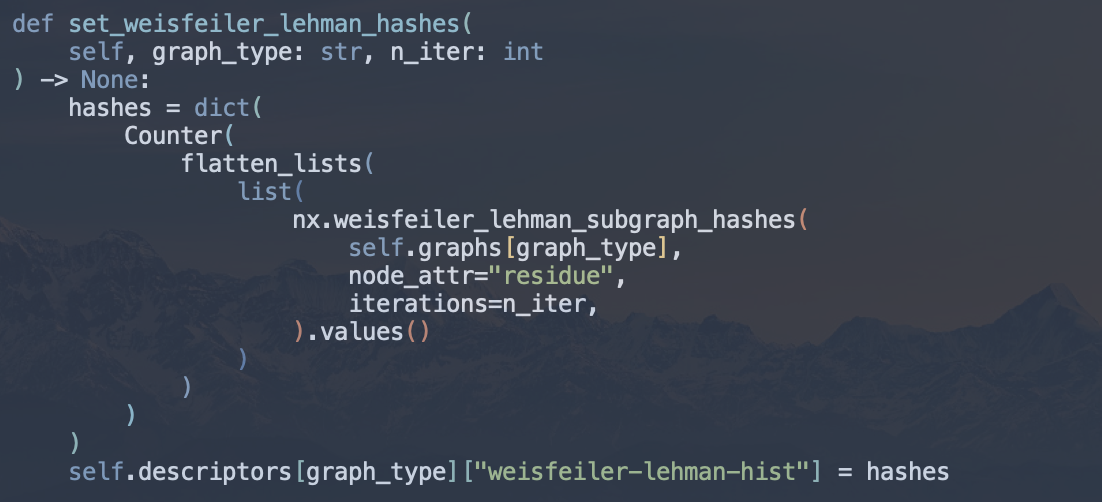
\includegraphics[width=.6\textwidth]{figures/setting_hash.png}
    \caption{Setting the hash histogram for each protein}
    \label{fig:hash_setting}
  \end{figure}
\end{frame}

\begin{frame}[fragile]{Weisfeiler-Lehmann kernel}
  What does the implementation look like?
  \begin{figure}
    \centering
    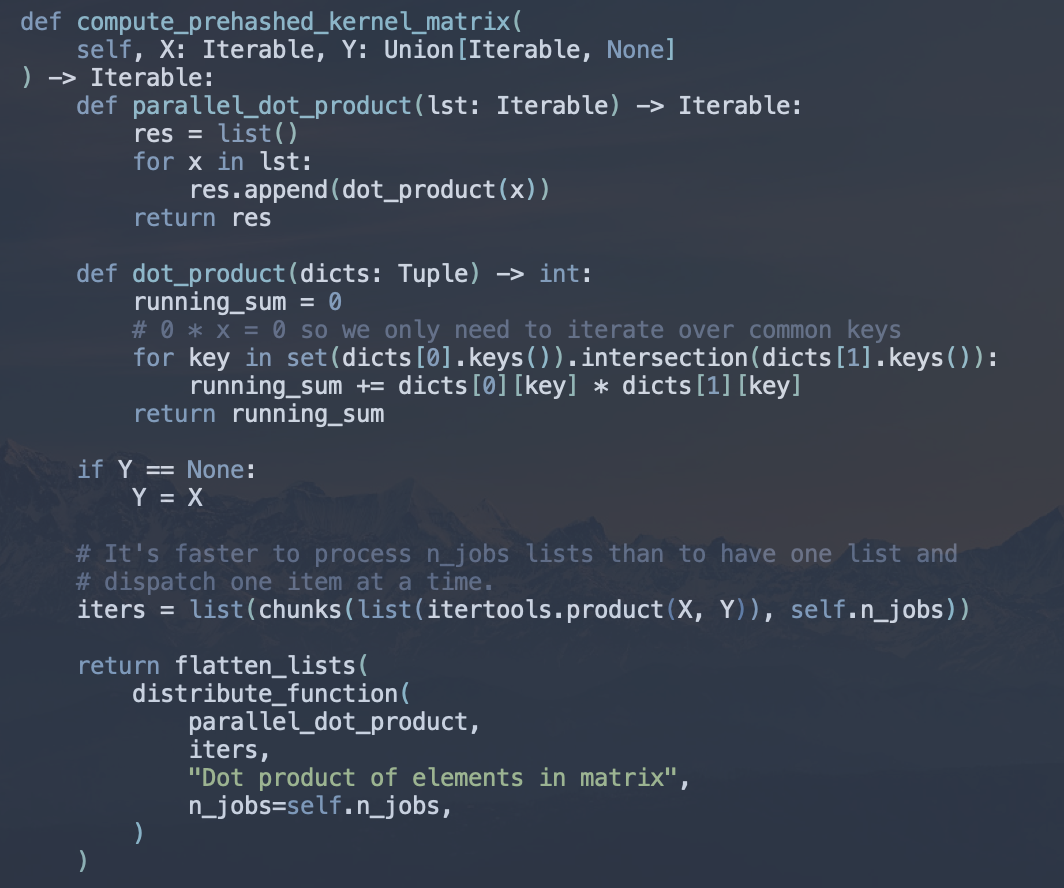
\includegraphics[width=.5\textwidth]{figures/dot_product.png}
    \caption{Computing the dot product of the feature maps in parallel.}
    \label{fig:hash_setting}
  \end{figure}
\end{frame}

\begin{frame}[fragile]{Weisfeiler-Lehmann kernel}
  How does it perform?
  \begin{figure}
    \centering
    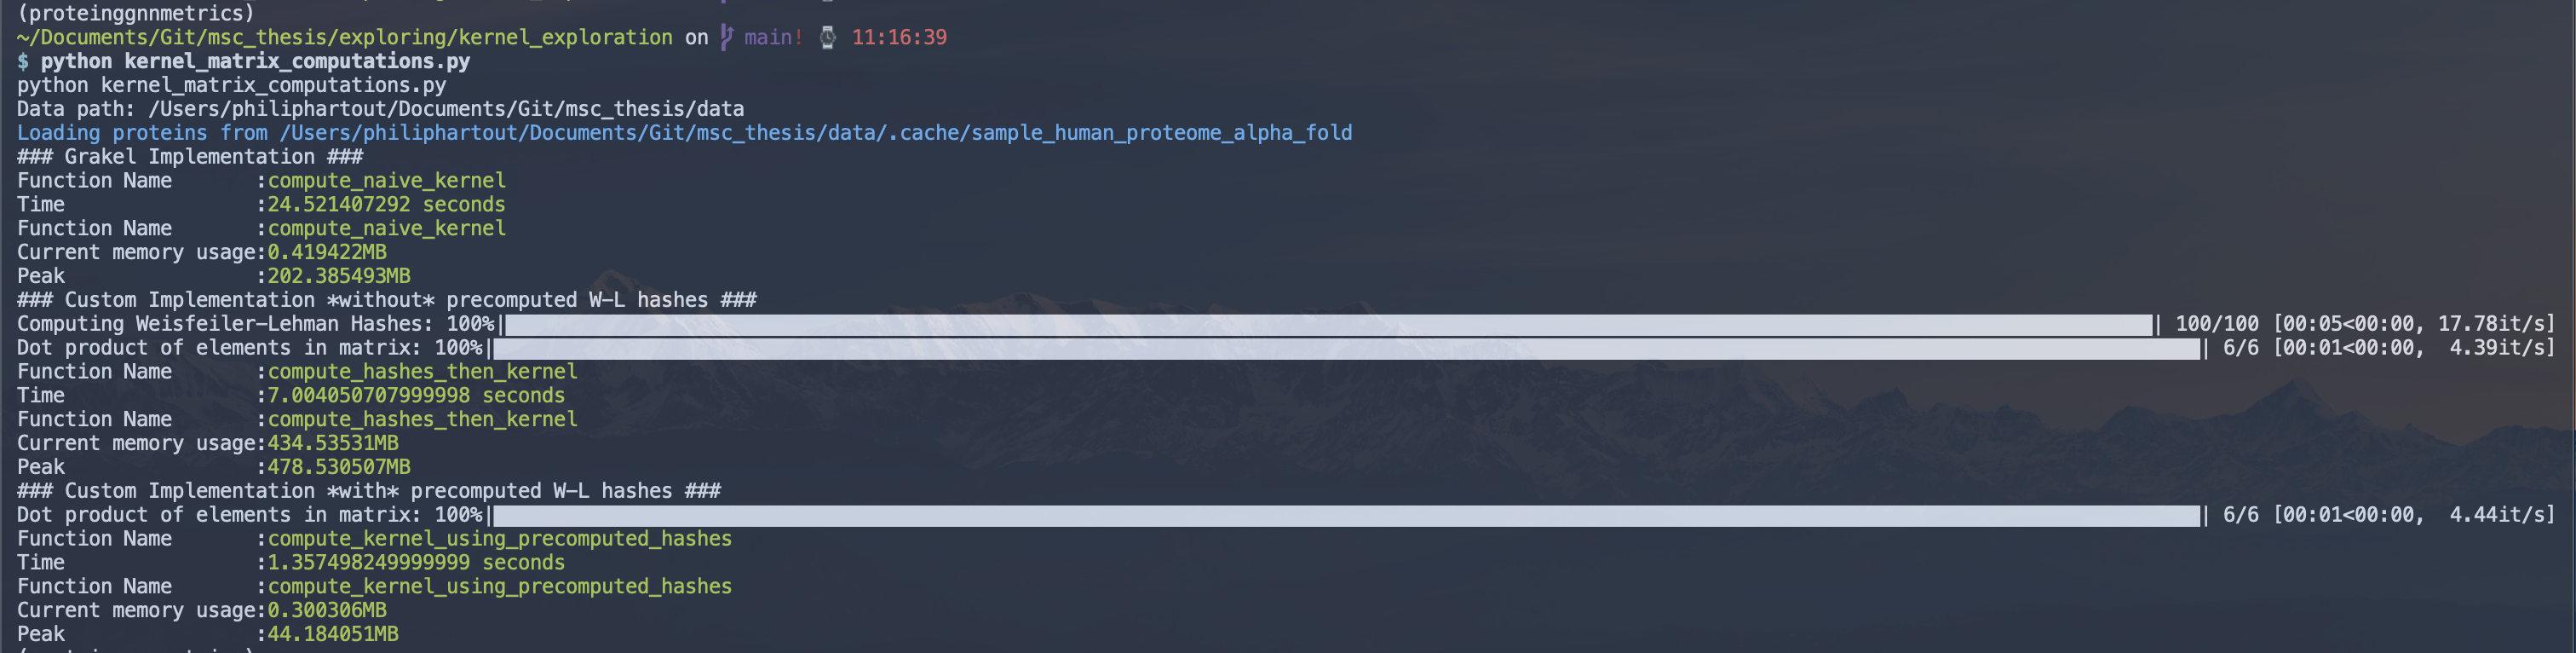
\includegraphics[width=\textwidth]{figures/wl-kernel_exec.png}
    \caption{Performance and memory footprint of grakel vs. custom. Both are
      done with 10 iterations of the W-L hashing step.}
    \label{fig:performance}
  \end{figure}
\end{frame}

\begin{frame}[fragile]{MMD}
  MMD implementations are different, why is the estimate more useful?\\
  \begin{minipage}{.45\textwidth}
  \begin{figure}
    \centering
    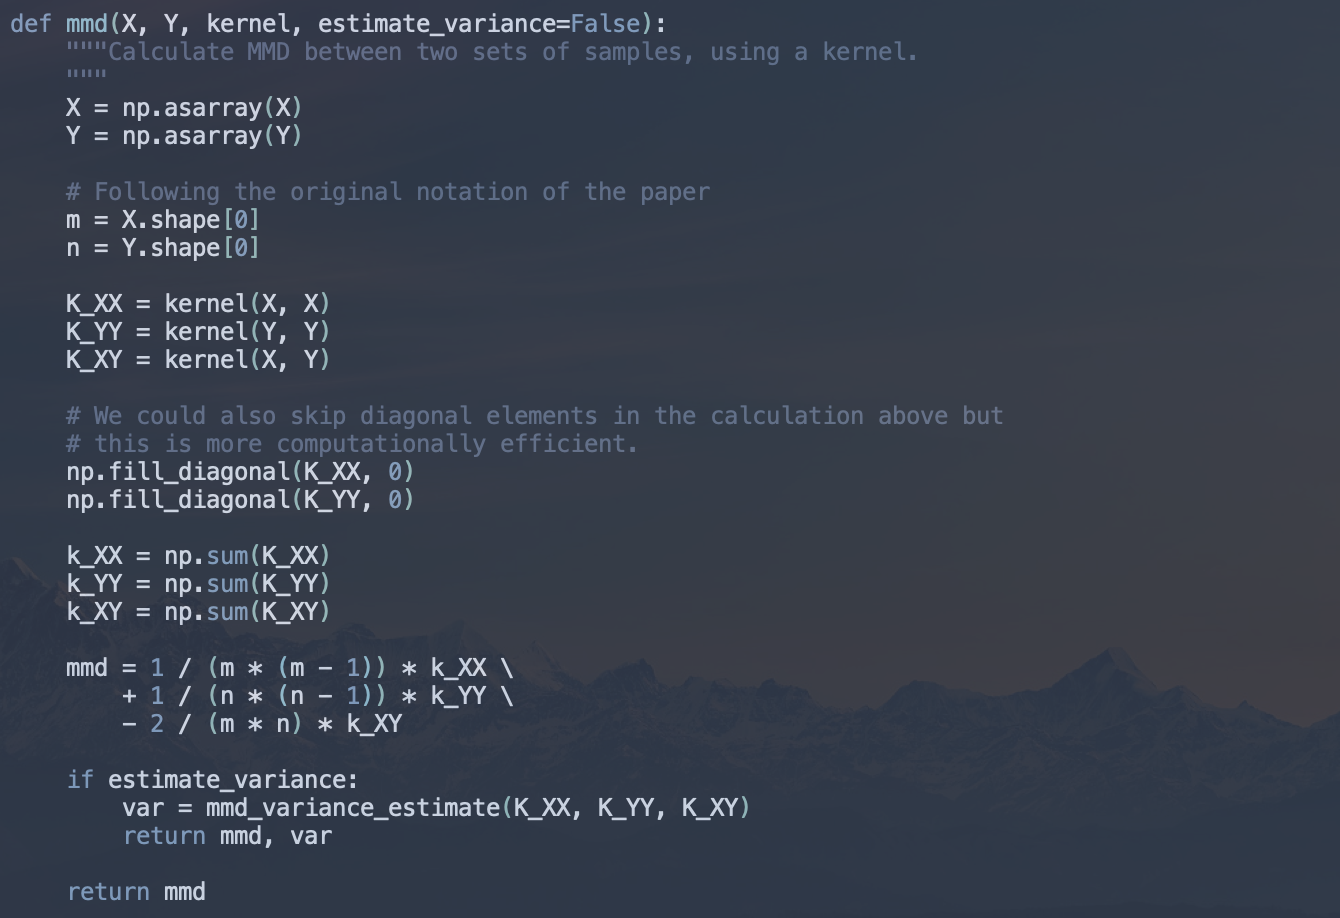
\includegraphics[width=\textwidth]{figures/mmd_estimate.png}
    \caption{MMD estimate, from ICLR \texttt{graphgeneval}}
    \label{fig:mmd_estimate}
  \end{figure}
  \end{minipage}%
  \hfill
  \begin{minipage}{.45\textwidth}
  \begin{figure}
    \centering
    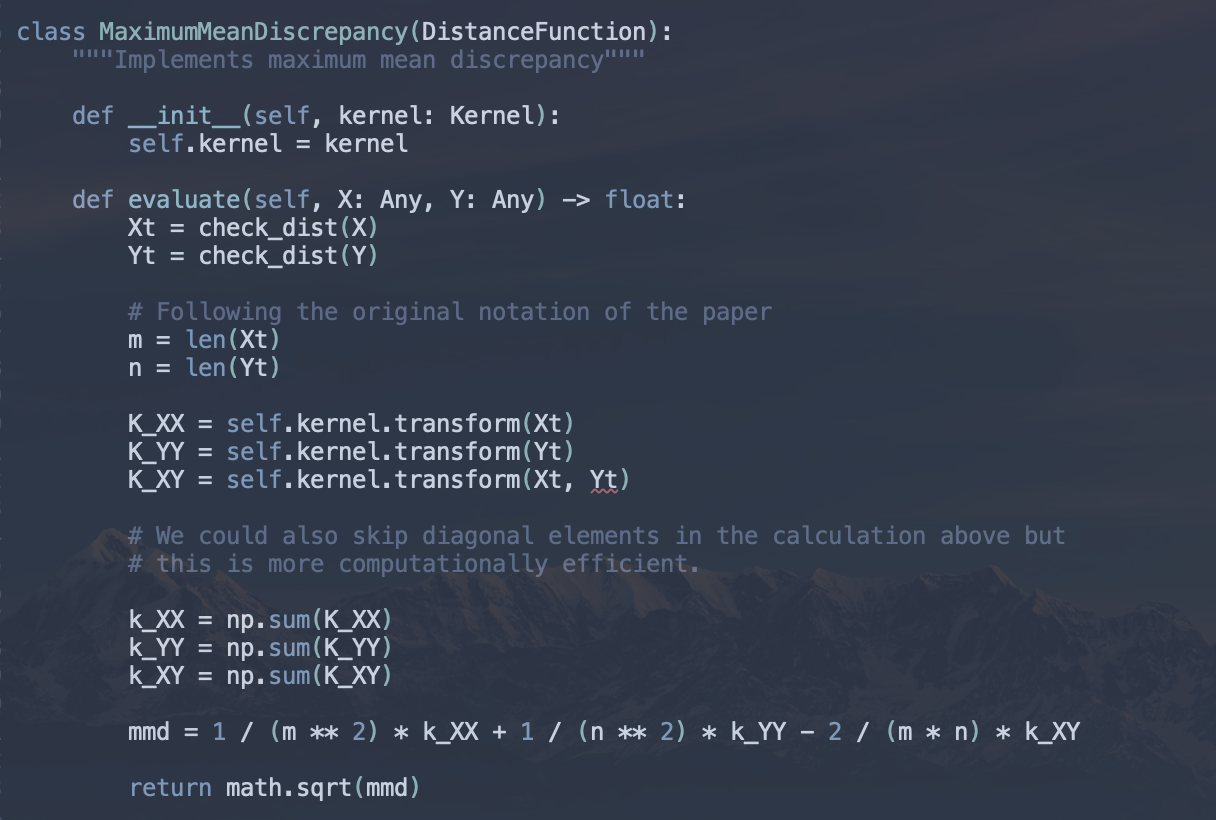
\includegraphics[width=\textwidth]{figures/mmd_current.png}
    \caption{MMD computation, from \texttt{proteinggnnmetrics}}
    \label{fig:mmd_current}
  \end{figure}
\end{minipage}
\end{frame}


\begin{frame}[fragile]{MMD}
  \begin{figure}
    \centering
    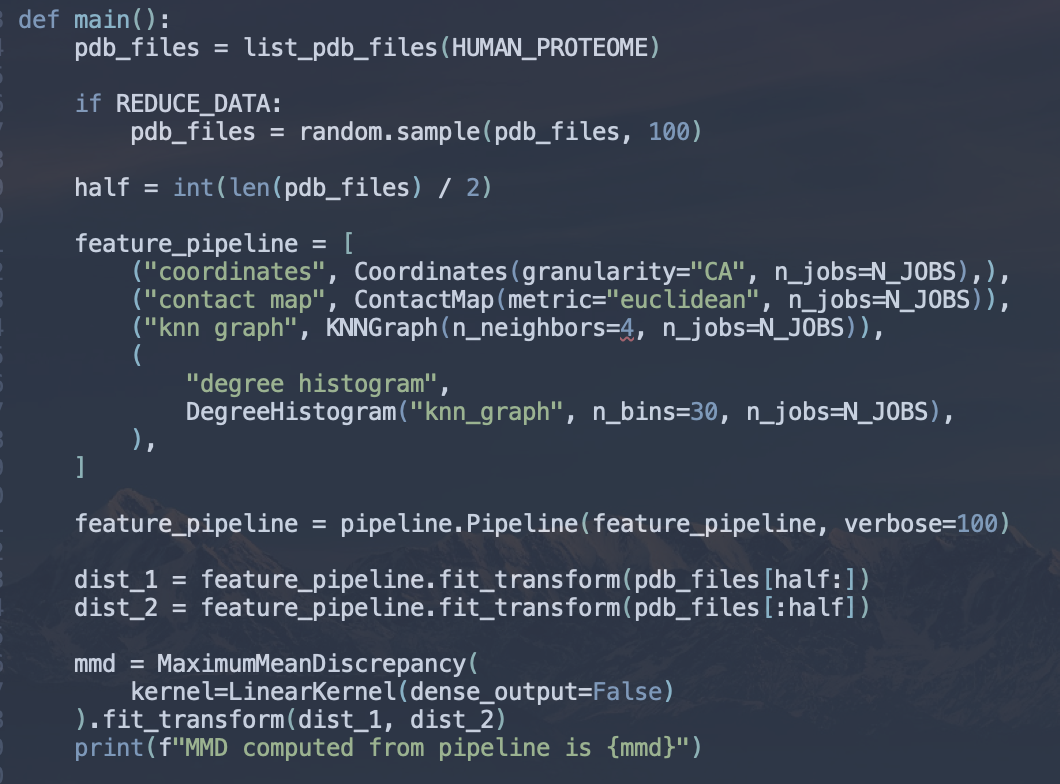
\includegraphics[width=0.5\textwidth]{figures/pipeline.png}
    \caption{Following \texttt{sklearn} standards}
    \label{fig:mmd_current}
  \end{figure}
\end{frame}


\begin{frame}[fragile]{Kernels for TDA features}
  The argument for using TDA features for MMD is that the (kernelized)
  descriptor functions needs to be ``rich enough''. TDA features are very
  expressive and operate on the contact map, a rich representation of any protein.
  \begin{figure}[center]
    \centering
    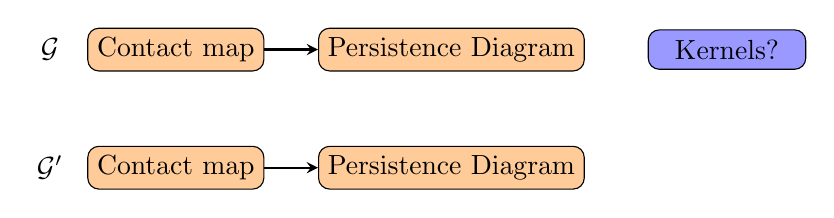
\begin{tikzpicture}[align=center, node distance=1.5cm, align=center]
      \node (cm0) [orangebox] {Contact map};
      \node (cm1) [orangebox, below of=cm0] {Contact map};
      \node (g) [left of=cm0, xshift=-0.1cm] {$\mathcal{G}$};
      \node (g_prime) [left of=cm1, xshift=-0.1cm] {$\mathcal{G}'$};
      \node (pd0) [orangebox, right of=cm0, xshift=2cm] {Persistence Diagram};
      \node (pd1) [orangebox, right of=cm1, xshift=2cm] {Persistence Diagram};
      \node (kernel) [bluebox, right of=pd0, xshift=2cm] {Kernels?};
      \draw [arrow] (cm0) -- (pd0);
      \draw [arrow] (cm1) -- (pd1);
    \end{tikzpicture}
    \caption{kernels on TDA features.}
    \label{fig:overview}
  \end{figure}
  Ideas: computer pairwise distances. Suppose persistence diagrams $\mathcal{P}_0,
  \mathcal{P}_1\sim\mathcal{G}$ and $\mathcal{P}_2, \mathcal{P}_3\sim\mathcal{G}'$.
  Can we do:
  $K_{W}(\mathcal{G},\mathcal{G}')=\begin{bmatrix}
    W_p(\mathcal{P}_0\mathcal{P}_2) & W_p(\mathcal{P}_1\mathcal{P}_2)\\
    W_p(\mathcal{P}_0\mathcal{P}_3) & W_p(\mathcal{P}_1\mathcal{P}_3)\\
  \end{bmatrix}$?\\
  Where $W_p(\mathcal{P},\mathcal{P}')$ is the $p$-Wasserstein distance between
  persistence diagrams. \\
  The Wasserstein distance \textit{is also a metric}. Some work by \cite{oh2019kernel} suggest this is more complex.
\end{frame}


\begin{frame}[fragile]{Motifs}
  Measure \textit{expressivity} of metric by comparing looking at proteins exhibiting
  structural motifs as a significant part of their structure. Example of motifs:
  \begin{itemize}
  \item Beta-hairpins
  \item Greek key
  \item Omega loop
  \item Helix-loop-helix
  \item Zinc fingers
  \item Helix-turn-helix
  \item Nest/niche
  \end{itemize}
\end{frame}

\begin{frame}[allowframebreaks]{References}

  \bibliography{../../thesis/refs.bib}
  \bibliographystyle{abbrv}

\end{frame}

\end{document}
